% created on 2019-12-13
% @author : bmazoyer

\chapter{Image spectral decomposition}



\section{The Heisenberg uncertainty principle in signal and image
processing}\label{the-heisenberg-uncertainty-principle-in-signal-and-image-processing}

The uncertainty principle is one of the most famous ideas in quantum mechanics. An early incarnation of the uncertainty principle appeared in a 1927 paper by the German physicist Heisenberg. The uncertainty principle says that we cannot measure the position $(x)$ and the momentum $(p)$ of a particle with absolute precision. The more accurately we know one of these values, the less accurately we know the other. 

However, the uncertainty principle in the field of quantum mechanics is just a particular case of a more general compromise that appears in many cases of everyday life involving waves. The central idea is connected with the interrelation between frequency and duration. For example, in the case of sound waves, if we want to identify the frequency of a musical note, the shorter the sound lasts in time, the less certain we can be about the exact frequency of the sound; to find a more defined frequency, it would be necessary to listen to the sound for a longer time. In the language of signal processing, we can say that a short signal correlates highly with a wide range of frequencies and only wide signals correlate with a short range of frequencies. Formally this is expressed as

\begin{equation}\label{eq:uncertainty_principle}
	(\Delta t)^2(\Delta \omega)^2 \geq \frac{1}{4}
\end{equation}

where $\Delta t$ is the duration of the signal in the time domain and $\Delta \omega$ is the bandwidth of the signal in the frequency domain (CITE). The uncertainty principle then says: the product of the spectral bandwidth multiplied with the time duration of the signal cannot be less than a certain minimum value.


The Heisenberg uncertainty principle in the field of signal processing and image processing can be mathematically proved by \textbf{Parseval's theorem}

\begin{equation}\label{eq:parseval_theorem}
	\int_{-\infty}^{\infty} f(t)^2 dt = \frac{1}{2 \pi} \int_{-\infty}^{\infty} |F(\omega)|^2 d\omega
\end{equation}

where $f(t)$ is a function and $F(\omega)$ its the Fourier transform. 

The \textbf{energy content} of the signal described by $f(t)$ is defined as:

\begin{equation}\label{eq:energy_content_time}
    E_{\infty} \equiv \int_{-\infty}^{\infty}  f(t)^2 dt
\end{equation}


From the Parseval's identity this may be written as:

\begin{equation}\label{eq:energy_content_frequency}
    E_{\infty} = \frac{1}{2 \pi} \int_{-\infty}^{\infty} |F(\omega)|^2 d\omega
\end{equation}

The \textbf{time dispersion} of the signal is given by

\begin{equation}\label{eq:time_dispersion_no_centered}
    (\Delta t)^2 \equiv \frac{1}{E_{\infty}} \int_{-\infty}^{\infty} (t-\bar{t})^2 f(t)^2 dt
\end{equation}


where if we shift the \textbf{center of gravity} of the signal to the origin $\bar{t}=0$, then

\begin{equation}\label{eq:time_dispersion}
    (\Delta t)^2 = \frac{1}{E_{\infty}} \int_{-\infty}^{\infty} t^2 f(t)^2 dt
\end{equation}

In an analogous way, the \textbf{spectral bandwidth} of the signal is given by

\begin{equation}\label{eq:spectral_bandwidth_no_centered}
    (\Delta \omega)^2 \equiv \frac{1}{2 \pi E_{\infty}} \int_{-\infty}^{\infty} (\omega-\bar{\omega})^2 |F(\omega)|^2 d\omega
\end{equation}

where if we consider an \textbf{spectral center of gravity}, $\bar{\omega}=0$

\begin{equation}\label{eq:spectral_bandwidth}
    (\Delta \omega)^2 = \frac{1}{2 \pi E_{\infty}} \int_{-\infty}^{\infty} \omega^2 |F(\omega)|^2 d\omega 
\end{equation}

If $f'(t)$ is the derivative of the function, its Fourier transform is $j\omega F(\omega)$. By applying the Parseval's theorem to the Fourier pair $f'(t)\longleftrightarrow j\omega F(\omega)$ we obtain:

\begin{equation}\label{eq:applyed_parseval_theorem}
    \int_{-\infty}^{\infty} \omega^2 |F(\omega)|^2 d\omega = 2 \pi \int_{-\infty}^{\infty} f'(t)^2 dt
\end{equation}

By substituting in equation $(\eqref{eq:spectral_bandwidth})$, we have:

\begin{equation}\label{eq:spectral_bandwidth2}
    (\Delta \omega)^2 = \frac{1}{E_{\infty}} \int_{-\infty}^{\infty} f'(t)^2 dt
\end{equation}

We use equations $(\eqref{eq:time_dispersion})$ and $\eqref{eq:spectral_bandwidth2}$ to calculate:

\begin{equation}\label{eq:time_bandwidth_disp}
    (\Delta t)^2(\Delta \omega)^2 = \frac{1}{E_{\infty}^{2}} \int_{-\infty}^{\infty} t^2f(t)^2 dt \int_{-\infty}^{\infty}f'(t)^2 dt
\end{equation}

Applying the Schwartz's inequality for the integrals on the right-hand side of $\eqref{eq:time_bandwidth_disp}$:

\begin{equation}\label{eq:schwartz_inequality}
    \int_{-\infty}^{\infty}tf(t)^2 dt \int_{-\infty}^{\infty}f'(t)^2 dt  \geq \biggr\rvert \int_{-\infty}^{\infty}tf(t)f'(t)^2 dt \biggr\rvert^{2}
\end{equation}


We may integrate by parts the integral on the right-hand side of $\eqref{eq:schwartz_inequality}$

\begin{equation}\label{eq:integr_by_parts}
    \int_{-\infty}^{\infty}tf(t)f'(t)^2 dt =  \frac{1}{2}tf(t)^2 \biggr\rvert_{\infty}^{\infty} - \frac{1}{2} \int_{-\infty}^{\infty}f(t)^2 dt
\end{equation}

If $\lim_{t\rightarrow \infty} tf(t)^2=0$, the first term on the right-hand side of $\eqref{eq:integr_by_parts}$ vanishes and from equation $\eqref{eq:energy_content_time}$ we have

\begin{equation}\label{eq:energy_content_developped}
    \int_{\infty}^{\infty} tf(t)f'(t) dt = -\frac{1}{2} E_{\infty}
\end{equation}

If we use this into $\eqref{eq:schwartz_inequality}$ and then into $\eqref{eq:time_bandwidth_disp}$ we obtain:

\begin{equation}\label{eq:}
   (\Delta t)^2(\Delta \omega)^2 \geq \frac{1}{4} 
\end{equation}

This is the mathematical statement of the uncertainty principle in signal processing.

\subsection{Examples}

The uncertainty principle shows that the size, the shape and the shift of the window through which we make measurements affects the accuracy of what we compute. For example, let us consider a signal $f(t)$ with Fourier transform $F(\omega)$. Let us assume that we observe only a part of the signal through a window $w(t)$, with Fourier transform $W(\omega)$ centered at $t_0$

\begin{equation}\label{eq:uncertainty_principle2}
    h(t) = f(t)w(t-t_0)
\end{equation}


Due to the shifting property of the Fourier transform, the Fourier transform of the window is $e^{-j\omega t_0}W(\omega)$. Since the window multiplies the signal, the Fourier transform of the window is convolved with the Fourier transform of the signal. Therefore, the Fourier transform of what we observe is given by:

\begin{equation}\label{eq:short_time_fourier_transform}
    H(\omega) = \int_{\infty}^{\infty}F(\omega - u)e^{-ju t_0}W(u) du
\end{equation}


In general $H(\omega)$ is different from $G(\omega)$ and depends on the locality of the window $t_0$.

To see this behavior, consider a signal $f(t)=A \sin \omega_{0} t$, where $A$ is a positive constant, and a window $w(t)$ defined by a Gaussian function. 

\begin{equation}\label{eq:1d_gaussian_function}
    w(t)=e^{-\frac{(t-t_0)^2}{2\sigma^2}}
\end{equation}
A Gaussian window is infinite in extent, so it is characterized by its locality $t_0$ and its standard deviation, which in this context is also called \textit{spread} and is denoted by $\sigma$. 

\begin{figure}
\centering
\subcaptionbox{}{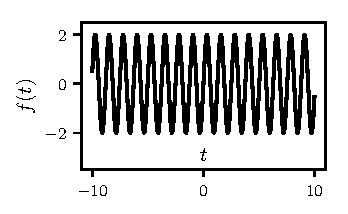
\includegraphics[width=0.325\textwidth]{sin_signal}\label{fig:sin_signal}}%
\subcaptionbox{}{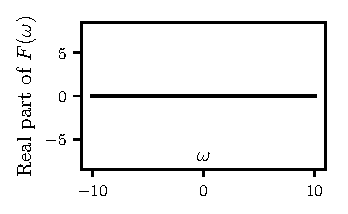
\includegraphics[width=0.325\textwidth]{real_sin_signal}}%\label{fig:sin_signal_real}
\subcaptionbox{}{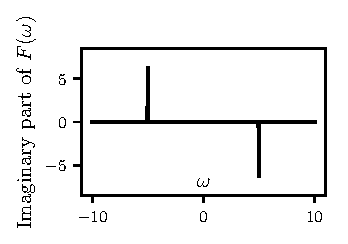
\includegraphics[width=0.325\textwidth]{imag_sin_signal}}\\%\label{fig:sin_signal_imag}
\hspace{0.33\textwidth}
\subcaptionbox{}{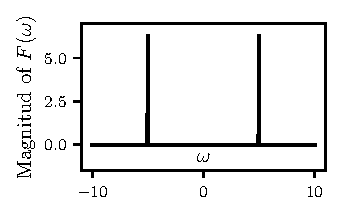
\includegraphics[width=0.325\textwidth]{mag_sin_signal}}%\label{fig:sin_signal_mag}
\subcaptionbox{}{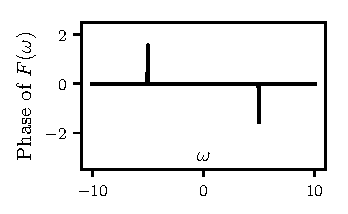
\includegraphics[width=0.325\textwidth]{phase_sin_signal}}%\label{fig:sin_signal_phase}
\caption{A continous fuction (a), and the real part (b), imaginary part (c), magnitude (d) and phase (e) of its Fourier transform}\label{fig:sin_signal_fourier_comp}
\end{figure}

Figures \ref{fig:sin_signal_fourier_comp, fig:gaussian_window_real_imag, fig:gaussian_window_mag_phase} demonstrate the result for a signal with $\omega_0=5$ and $A=2$. Figure \ref{fig:sin_signal_fourier_comp} shows the continuous signal and  the real and imaginary parts and the magnitude and phase of its Fourier transform.  Figure \ref{fig:gaussian_window_real_imag} shows various windowed parts of the signal ($h(t)$) and the real and imaginary parts of their corresponding Fourier transforms.  Figure \ref{fig:gaussian_window_mag_phase} is the same as figure \ref{fig:gaussian_window_real_imag}, but it shows the magnitude and phase of each Fourier transform. These Fourier transforms should be compared with their counterparts in figure \ref{fig:sin_signal_fourier_comp} in order to appreciate the effect of both the size of the window and the locality of the window (Gaussian function). In all cases the main peaks of the Fourier transform's magnitude, which correspond to delta function impulses at $\omega=\pm 5$ in the continuous case, are preserved, but they become less sharp and the recovered value starts to move away from the real value as soon as the size of the window decreases. 



\begin{figure}
\centering
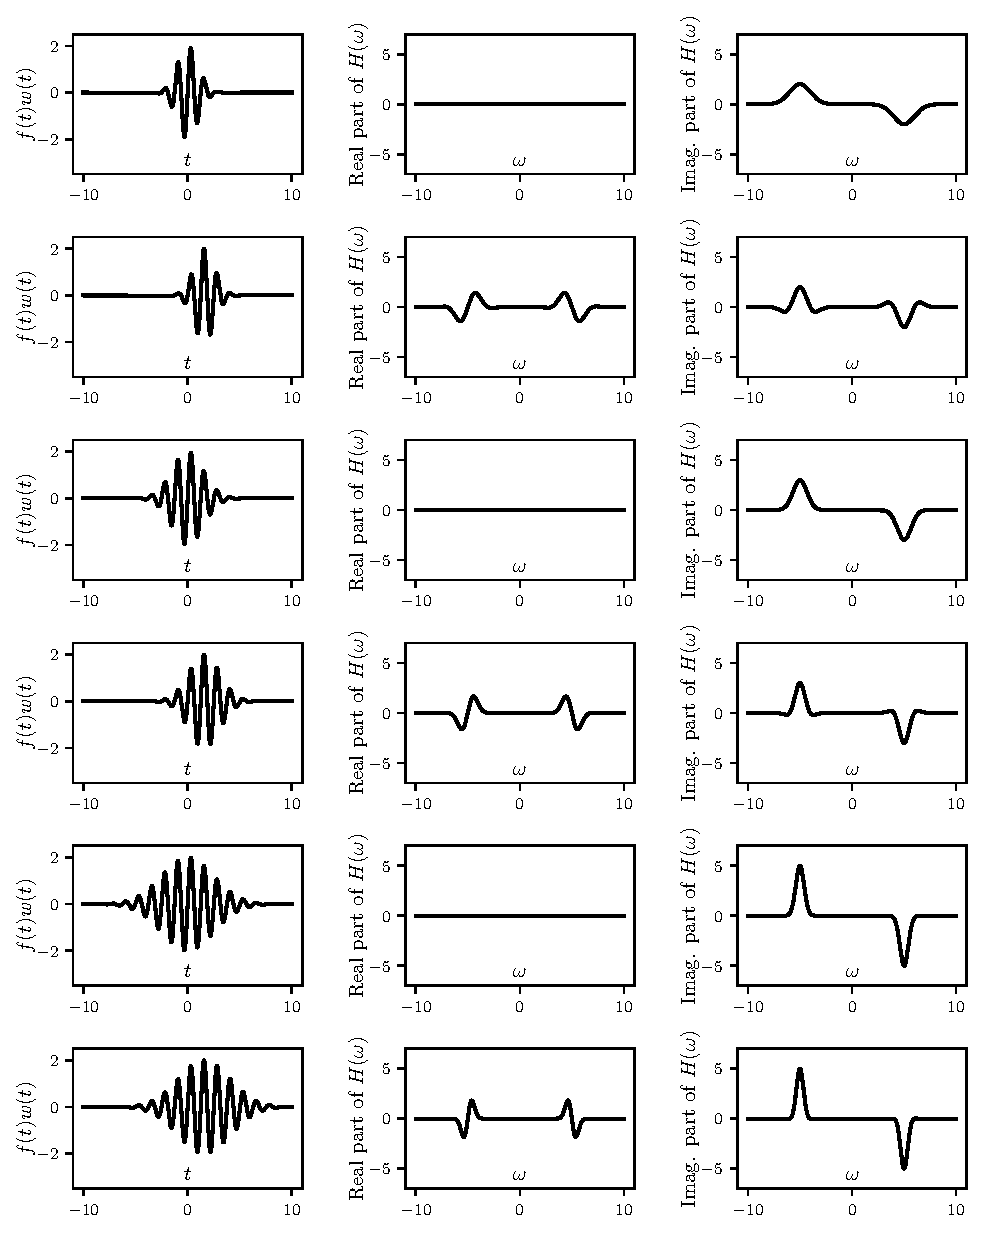
\includegraphics{sin_gauss_real_imag.pdf}
\caption{The effect of Gaussian window. Sinusoidal signal bounded by a Gaussian window (first column) and the real and imaginary part of its corresponding Fourier transform (second and third columns). From top to bottom: $[\sigma=1, t_0=0]$, $[\sigma=1, t_0=1.6]$, $[\sigma=1.5, t_0=0]$, $[\sigma=1.5, t_0=1.6]$, $[\sigma=2.5, t_0=0]$, $[\sigma=2.5, t_0=1.6]$}\label{fig:gaussian_window_real_imag}
\end{figure}

\begin{figure}
\centering
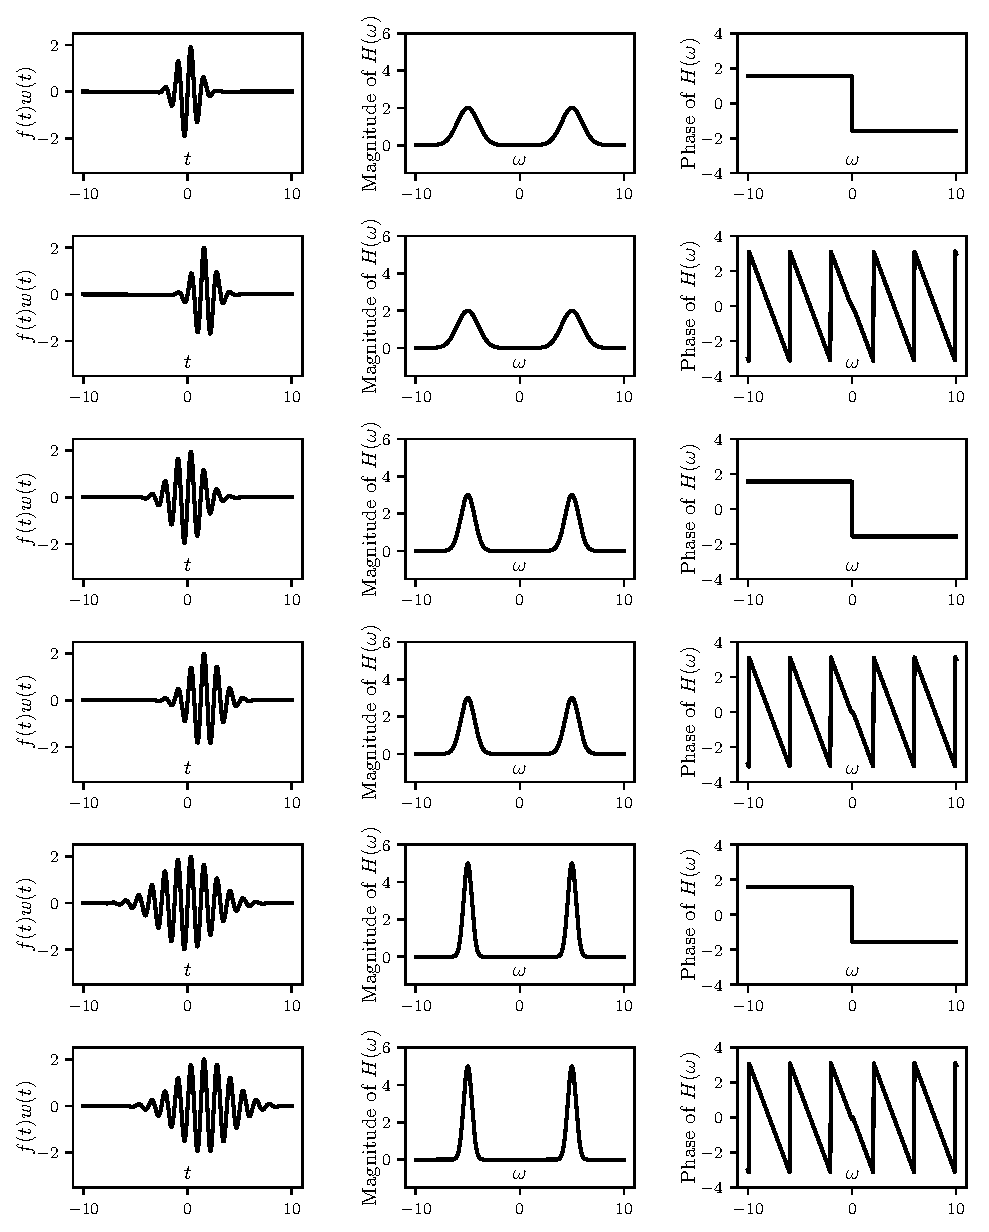
\includegraphics{sin_gauss_mag_phase.pdf}
\caption{The effect of Gaussian window. Sinusoidal signal bounded by a Gaussian window (first column) and the magnitude and phase of its corresponding Fourier transform (second and third columns). From top to bottom: $[\sigma=1, t_0=0]$, $[\sigma=1, t_0=1.6]$, $[\sigma=1.5, t_0=0]$, $[\sigma=1.5, t_0=1.6]$, $[\sigma=2.5, t_0=0]$, $[\sigma=2.5, t_0=1.6]$}\label{fig:gaussian_window_mag_phase}
\end{figure}






